%%%%%%%%%%%%%%%%%%%%%%%%%%%%%%%%%%%%%%%%%%%%%%%%%%%%%%%%%%%%%%%%%%%%%%%%%%%%%%%%
% simulation.tex: Chapter on MC production:
%%%%%%%%%%%%%%%%%%%%%%%%%%%%%%%%%%%%%%%%%%%%%%%%%%%%%%%%%%%%%%%%%%%%%%%%%%%%%%%%
\chapter{Digital Storage System and IO Workload}
\label{storage}
%%%%%%%%%%%%%%%%%%%%%%%%%%%%%%%%%%%%%%%%%%%%%%%%%%%%%%%%%%%%%%%%%%%%%%%%%%%%%%%%
\begin{figure}[h]
\centering
%\begin{tikzpicture}[node distance = 0.85in, auto]
%\draw[style=dashed] (2,.5) circle (0.5);
%\end{tikzpicture}
%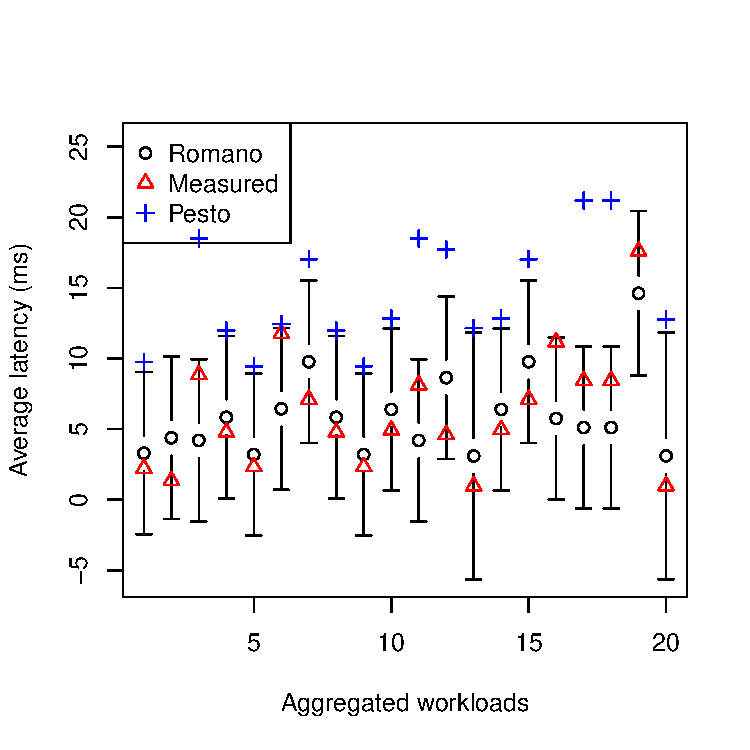
\includegraphics{figure/aggr_result.pdf}
%\begin{tikzpicture}[show background grid, auto]
\begin{tikzpicture}[auto]
\node[ellipse,
			%cylinder,
			%shape border rotate = 90,
			%aspect = 0.25,
			minimum height = 2cm,
			draw] (Storage) {
				Storage System
			}; 
\draw (Storage.north west) -- (-2,1.5) -- (-2.5,1.5) node[left]{Flexibility};
\draw (Storage.south west) -- (-2,-1.5) -- (-2.5,-1.5) node[left]{Capacity};
\draw (Storage.north east) -- (2,1.5) -- (2.5,1.5) node[right]{Power};
\draw (Storage.south east) --(2,-1.5) -- (2.5,-1.5) node[right]{Reliability};
\draw (Storage.south) -- (0,-1.5)	node[below]{Performance};
\draw[-triangle 90] (-0.7, 2)node[above]{Store} -- (Storage.110);
\draw[-triangle 90] (Storage.70) -- (0.7, 2)node[above]{Load};
\end{tikzpicture}

\caption{Storage system operation and attributes.}
\label{fig:storageAttribute}
\end{figure}
A storage system is a system that supports two operations, \emph{load} and \emph{store}. 
The \emph{load} operation allows system to change its internal state and the \emph{store} operation allows this state to be verified. 
A storage system must further ensure that the interval state is immutable in an absence of a \emph{store} operation.

There are five types of attributes which defines a storage system. 
The first type of attributes, \emph{flexibility} attribute, describe the allowed state transitions. 
A generic storage system allows all states to be reached from every other state and will be the focus of this thesis. 
The second type of attribute, \emph{capacity} attribute is the number of the states and defines the storage \emph{capacity}.
The third type of attribute, \emph{power} attribute, defines power requirement for maintaining the states, state transition and state verification. 
The fourth type of attribute, \emph{reliability} defines the probability of state transition in the absence of \emph{store} operation. 
The last attribute, \emph{performance} attribute, defines speed at which the state transitions occur as well as verification of the states. 
These classification of attributes as well as the two primary operations are shown in Figure \ref{fig:storageAttribute}.

These attributes can again be grouped into two types. 
The first type is operation independent. 
They maybe affected by other source of stress such as the temperature but are largely unaffected by the operations to which the system is exposed. 
The second type is operation dependent. 
These attributes define the interaction between the storage systems and the operations and typically results in side effects that is not a required result of \emph{load} and \emph{store} operations. 

Quantifying those side effect is the true goal of this thesis with a special focus on the performance attribute.

\section{Digital Storage System}
\begin{table}[t]
\centering
\begin{tabular}{p{1.3cm}||p{2.1cm}|p{2.1cm}|p{2.1cm}|p{2.1cm}|p{2.1cm}}
\hline
\hline
 			& Flexibility & Capacity & Power & Reliability & Performance \\
\hline
\hline
Punch Card		& \raggedright{Bits can only be set and cannot be unset}
							&	\raggedright{$<10$ bits per $in^2$}
							&	\raggedright{$0$ Watts for state maintenance} 
							&	\raggedright{Wear and tear}
							&	2Kbps write, 4Kbps read 
\\
\hline
Hard Disk			& & & & & \\
\hline
NAND Flash		&	&	&	&	&	\\
\hline
PCM						&	&	&	&	&	\\
\hline
\hline
\end{tabular}
\caption{Various digital storage technologies and their attributes.}
\label{tbl:medium}
\end{table}
A digital storage system represents its internal state in a sequence of binary digits. 
The underlying storage medium that allows these digital storage systems have diversified in recent years. 


%%%%%%%%%%%%%%%%%%%%%%%%%%%%%%%%%%%%%%%%%%%%%%%%%%%%%%%%%%%%%%%%%%%%%%%%%%%%%%%%
